% Down-and-out put, coin exclu : les trois constructions de g2 sont indiscernables
% à cinq graines, et leur erreur commune est le plancher du défaut de trace
% terminale. Figures et chiffres tirés des artefacts sauvegardés des runs du
% 12--14 septembre 2026 (aucun nouvel entraînement). Compilable tel quel (pdfLaTeX).
\documentclass[11pt]{article}

\usepackage[a4paper,margin=0.9in]{geometry}
\usepackage[T1]{fontenc}
\usepackage[utf8]{inputenc}
\usepackage[french]{babel}
\usepackage{amsmath,amssymb}
\usepackage{booktabs}
\usepackage{graphicx}
\usepackage{xcolor}
\usepackage[hyphens]{url}
\usepackage[colorlinks=true,allcolors=blue!55!black]{hyperref}
\urlstyle{tt}
\sloppy

\newcommand{\epscoin}{\varepsilon_{\mathrm{coin}}}
\newcommand{\etabli}{\textbf{[ÉTABLI]}}
\newcommand{\mesure}{\textbf{[MESURÉ]}}
\newcommand{\LBS}{\mathcal L^{BS}}
\newcommand{\VDO}{V_{DO}}
\newcommand{\code}[1]{\texttt{#1}}
\DeclareUrlCommand\codepath{\urlstyle{tt}}

\title{Down-and-out put, coin exclu de la collocation :\\
\large les trois constructions de $g_2$ sont indiscernables à cinq graines,\\
et leur erreur commune est le plancher du défaut de trace terminale}
\author{}
\date{14 septembre 2026}

\begin{document}
\maketitle

\section*{Cadre}

Contrat $K=1$, $B=0.6$, $r=0.03$, $\sigma=0.3$, $T=1$, domaine tronqué
$\Omega=(B,s_\infty)\times(0,T)$ avec $s_\infty=3$. Solution d'essai
$\Phi_\theta=g_1u_\theta+g_2$, $g_1(s,t)=(T-t)(s-B)$,
$g_2(s,t)=\zeta\big(\tfrac{s-B}{\epscoin}\big)\,h(s,t)$ avec $\epscoin=0.1$ et
$\zeta$ le plateau $C^\infty$ de la Définition 5. Trois \emph{constructions de
$g_2$}, c'est-à-dire trois choix de $h$ avec $h(s,T)=(K-s)^+$ : $h=V^e$ (prix
Black-Scholes du put européen), entraîné avec l'assemblage ordinaire du résidu
et avec l'assemblage à deux termes $\LBS(g_1u_\theta)+\LBS g_2$ ; $h=\pi$
(profil split-semigroupe, $\sigma_c=\sigma$, $n_{\mathrm{quad}}=8000$),
assemblage à deux termes. Quinze runs : $5$ graines maîtresses par
construction, $50\,000$ itérations, $n_f=4096$ points de collocation par pas
tirés uniformément sur $\Omega$ moins le triangle
$N_{0.1}=\{(s-B)+(T-t)\le0.1\}$, $4$ threads, hôte \code{republique}
(AVX2), commits \code{efbb9a8}/\code{ca3a630} (split) et \code{5e3c6f5}
(Black-Scholes). Référence $\VDO$ : forme close de Reiner-Rubinstein.
Sauf mention contraire, $\|\cdot\|$ désigne la norme $L^2$ discrétisée sur la
grille de mesure indiquée, et l'erreur relative est
$\|\Phi_\theta-\VDO\|/\|\VDO\|$ (respectivement avec $\partial_s$,
$\partial_{ss}$). Toutes les figures sont reconstruites à partir des artefacts
sauvegardés (fichiers \code{.yaml} voisins), sans réentraînement.

\section{Les trois constructions sont indiscernables}

\begin{figure}[htbp]
\centering
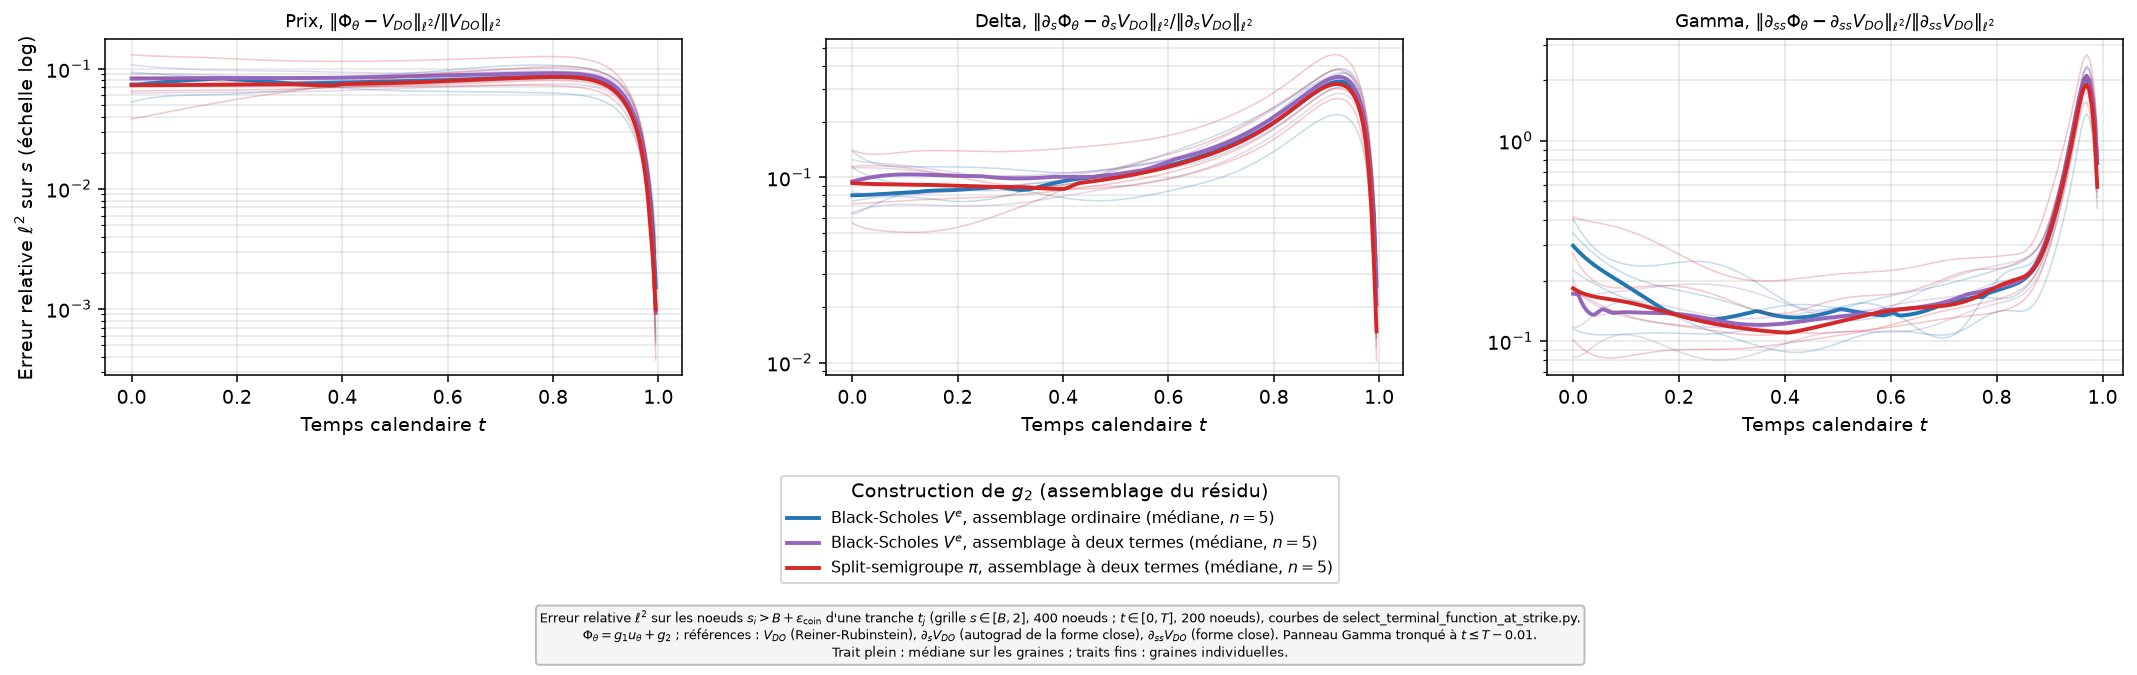
\includegraphics[width=\linewidth]{figures/fig1_erreur_vs_temps_median.png}
\caption{\mesure\ Figure « erreur vs temps » du rapport de sélection,
répliquée à cinq graines par le même script
(\codepath{select_terminal_function_at_strike.py}). Erreur relative $\ell^2$
sur les noeuds $s_i>B+\epscoin=0.7$ d'une tranche $t_j$ (grille
$s\in[B,2]$, $400$ noeuds ; $t\in[0,T]$, $200$ noeuds) du prix, du Delta et
du Gamma. Trait plein : médiane sur les graines ; traits fins : graines.
Les trois médianes coïncident à l'épaisseur du trait près sur les trois
panneaux et à tout $t$ ; le faisceau des graines d'une construction contient
les médianes des deux autres.}
\label{fig:erreur-vs-temps}
\end{figure}

\begin{figure}[htbp]
\centering
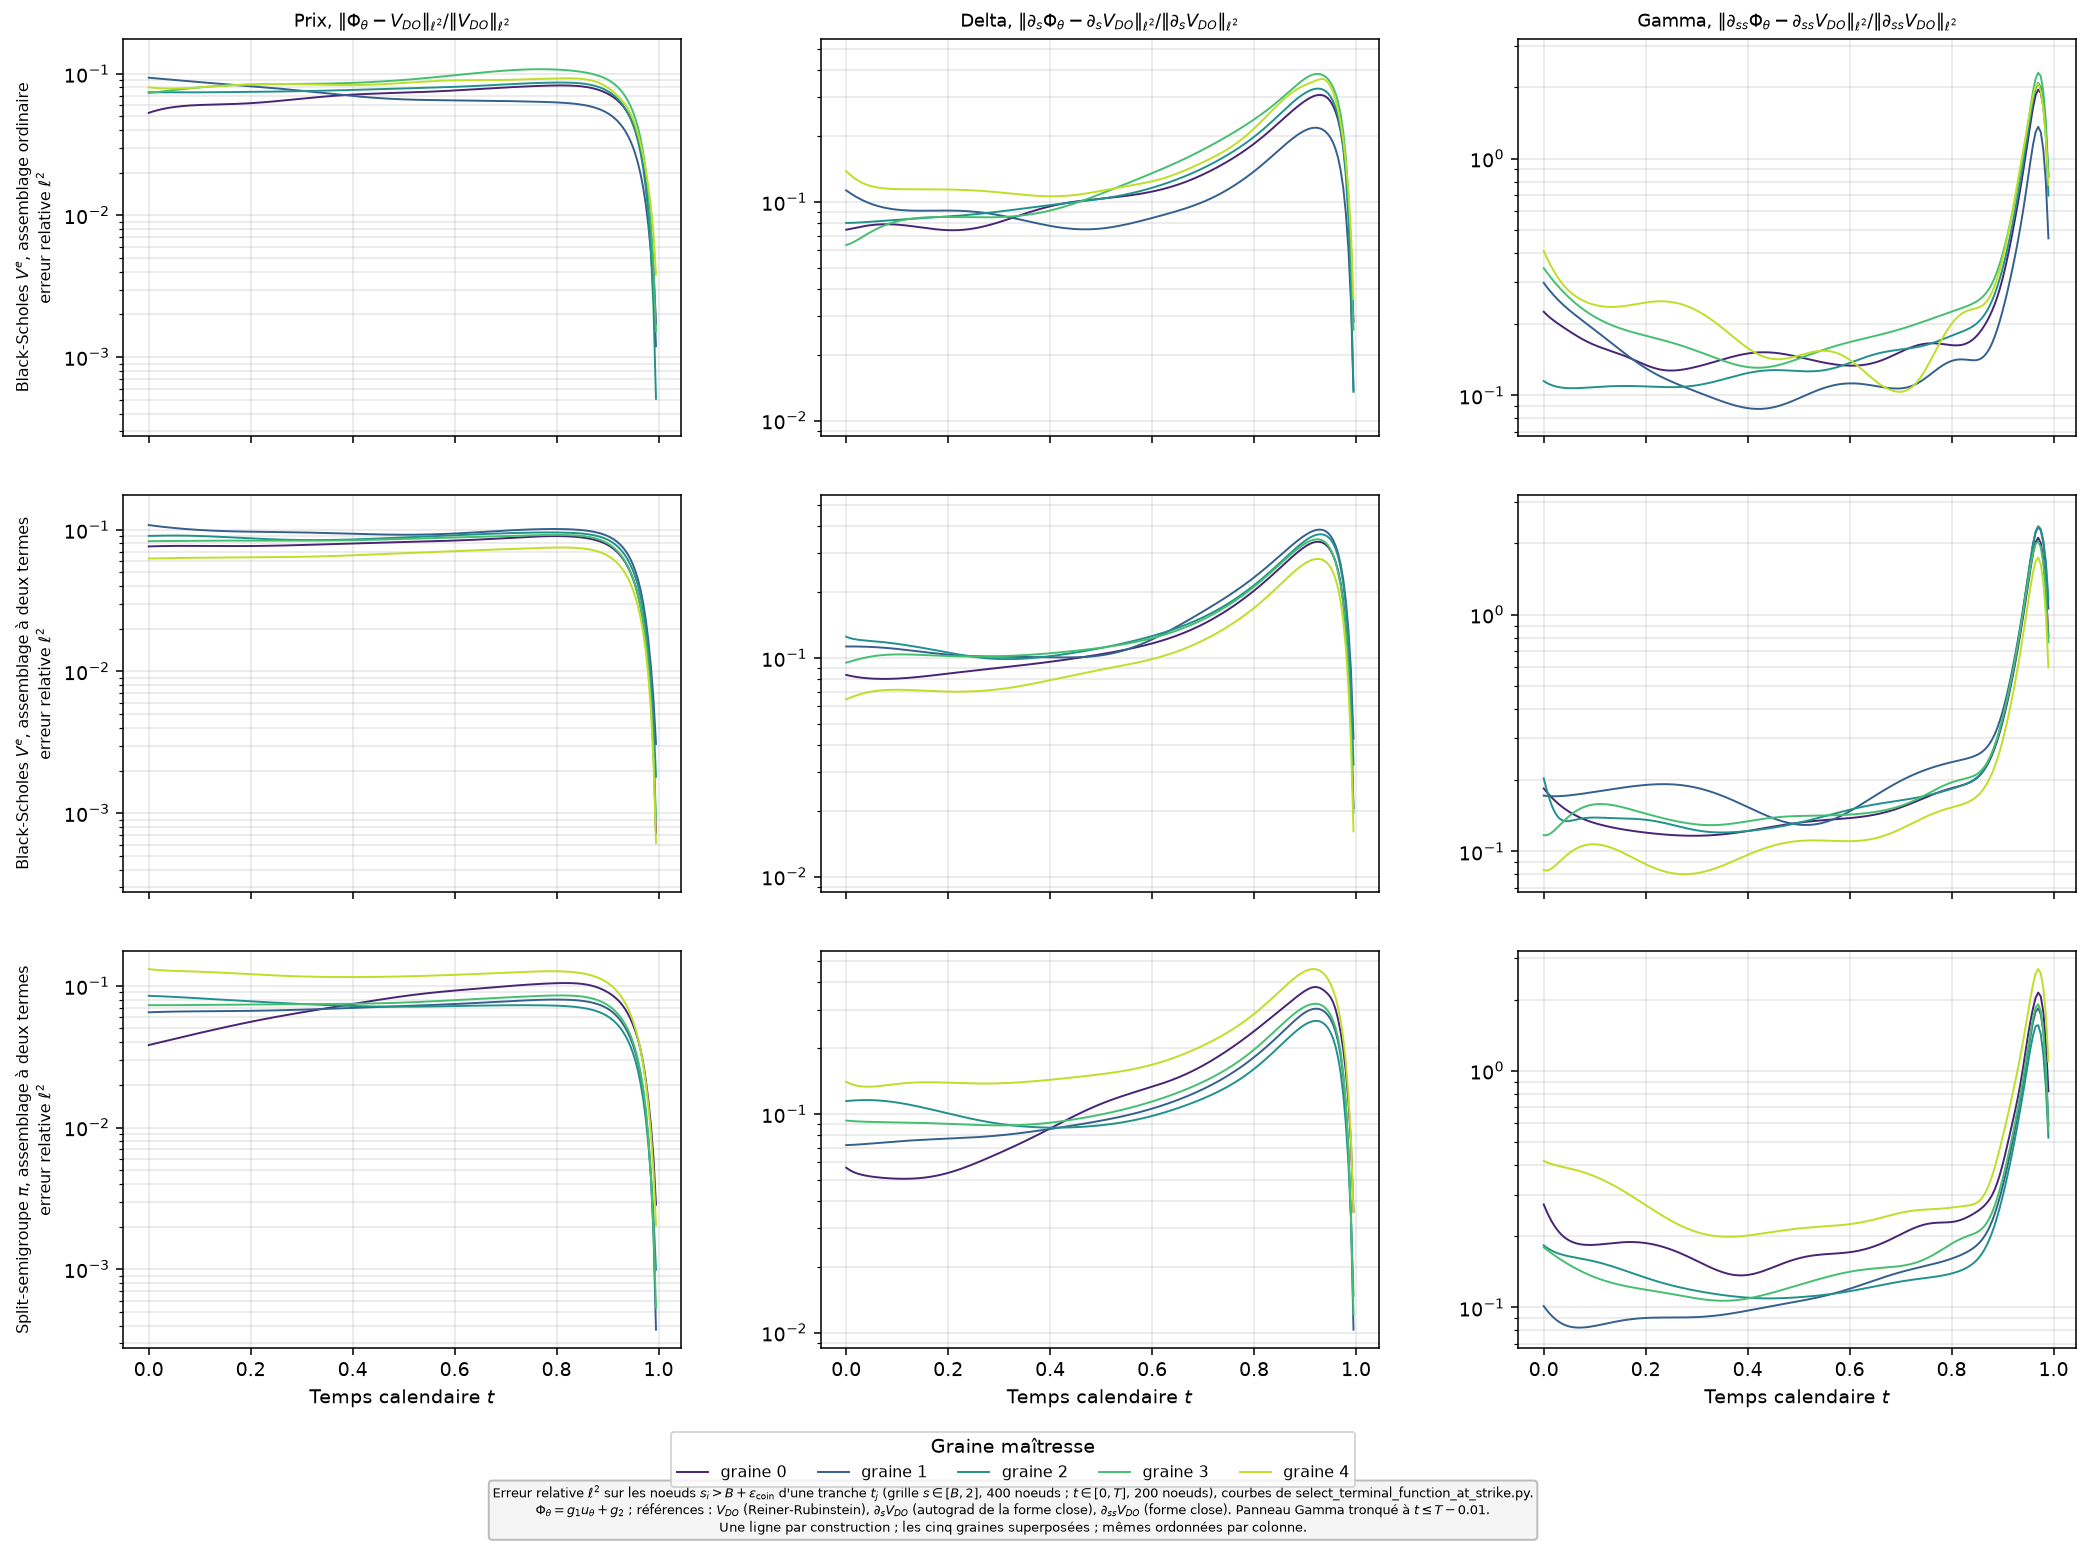
\includegraphics[width=\linewidth]{figures/fig1b_erreur_vs_temps_par_construction.png}
\caption{\mesure\ Mêmes courbes, une ligne par construction, les cinq graines
superposées, mêmes ordonnées par colonne. Dispersion entre graines d'une même
construction : facteur $\simeq1.5$ sur le prix, $\simeq2$ sur le Gamma, à
comparer aux écarts entre médianes de la figure~\ref{fig:erreur-vs-temps}.}
\label{fig:par-construction}
\end{figure}

\begin{figure}[htbp]
\centering
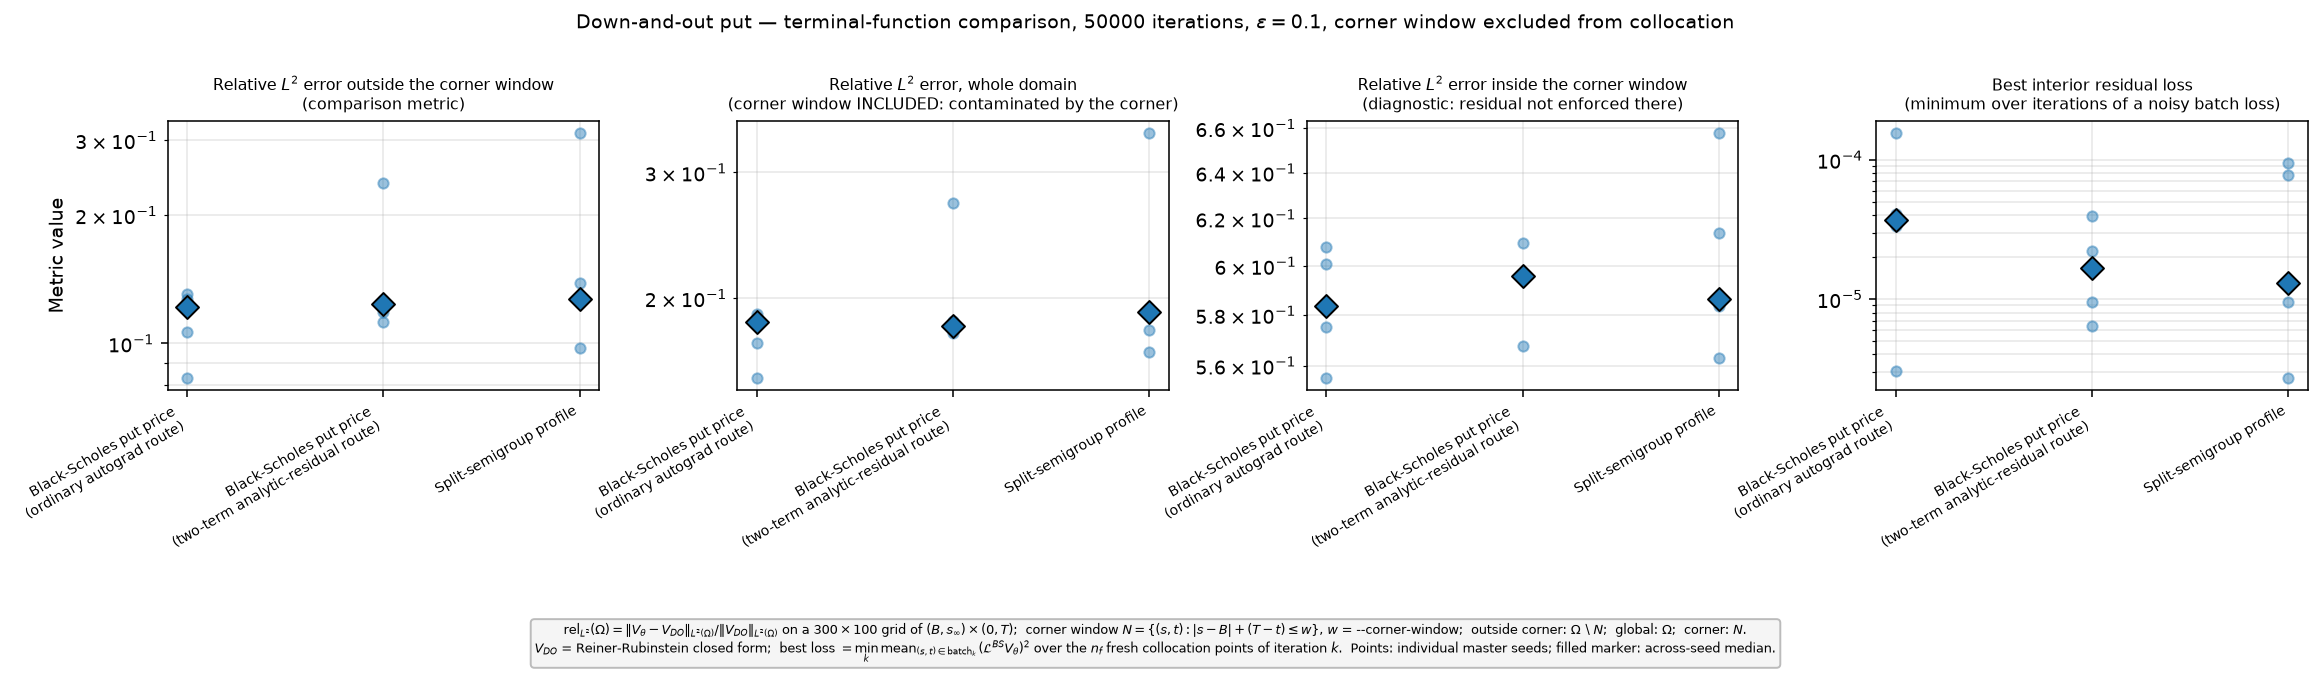
\includegraphics[width=\linewidth]{figures/fig2_comparaison_par_graine.png}
\caption{\mesure\ Métriques par graine (points) et médiane (losange) sur le
domaine $\Omega$ entier ($300\times100$ noeuds) : erreur relative hors
fenêtre du coin $\Omega\setminus N_{0.1}$ (métrique de comparaison), erreur
relative globale (fenêtre incluse, contaminée par la discontinuité du coin),
erreur relative dans la fenêtre (diagnostic), meilleur loss intérieur. Les
intervalles [min, max] des trois constructions se recouvrent pour chaque
métrique ; le meilleur loss du split est $3$ fois plus bas sans que son erreur
le soit.}
\label{fig:par-graine}
\end{figure}

\paragraph{Chiffres.} \mesure\ Médiane sur cinq graines [min, max] :

\begin{center}
\small
\begin{tabular}{@{}lccc@{}}
\toprule
Construction (assemblage) & $\|\Phi_\theta-\VDO\|/\|\VDO\|$ sur $\Omega\setminus N_{0.1}$ & Delta sur $\{s>0.7\}$ & Gamma sur $\{s>0.7\}$, $t\le T-0.2$ \\
\midrule
Black-Scholes $V^e$ (ordinaire) & $0.122$ [$0.083$, $0.130$] & $0.205$ [$0.140$, $0.239$] & $0.151$ [$0.119$, $0.185$] \\
Black-Scholes $V^e$ (deux termes) & $0.124$ [$0.113$, $0.237$] & $0.216$ [$0.175$, $0.240$] & $0.155$ [$0.120$, $0.187$] \\
Split $\pi$ (deux termes) & $0.127$ [$0.098$, $0.311$] & $0.199$ [$0.166$, $0.287$] & $0.145$ [$0.126$, $0.247$] \\
\bottomrule
\end{tabular}
\end{center}

\noindent Pour chacune des trois quantités, l'écart entre les médianes
extrêmes ($4$ pour cent sur le prix, $8$ sur le Delta, $7$ sur le Gamma) est
inférieur à l'étendue entre graines de chaque construction prise seule
(facteur $1.6$ à $3.2$). À $n=5$, aucune différence entre constructions n'est
établie sur la précision.

\paragraph{Pourquoi la version précédente classait.} Le rapport de sélection
comparait un run par construction (graine $0$, $20\,000$ itérations, coin non
exclu), sur des runs répartis entre deux machines et sans nombre de threads
enregistré ; les écarts qu'il ordonnait ($10$ à $50$ pour cent) sont de
l'ordre de la dispersion entre graines mesurée ici. Le classement n'était pas
reproductible ; il n'est pas contredit par une mesure plus fine, il n'était
pas résolu.

\section{Leur erreur commune est un plancher, et il est expliqué}

\begin{figure}[htbp]
\centering
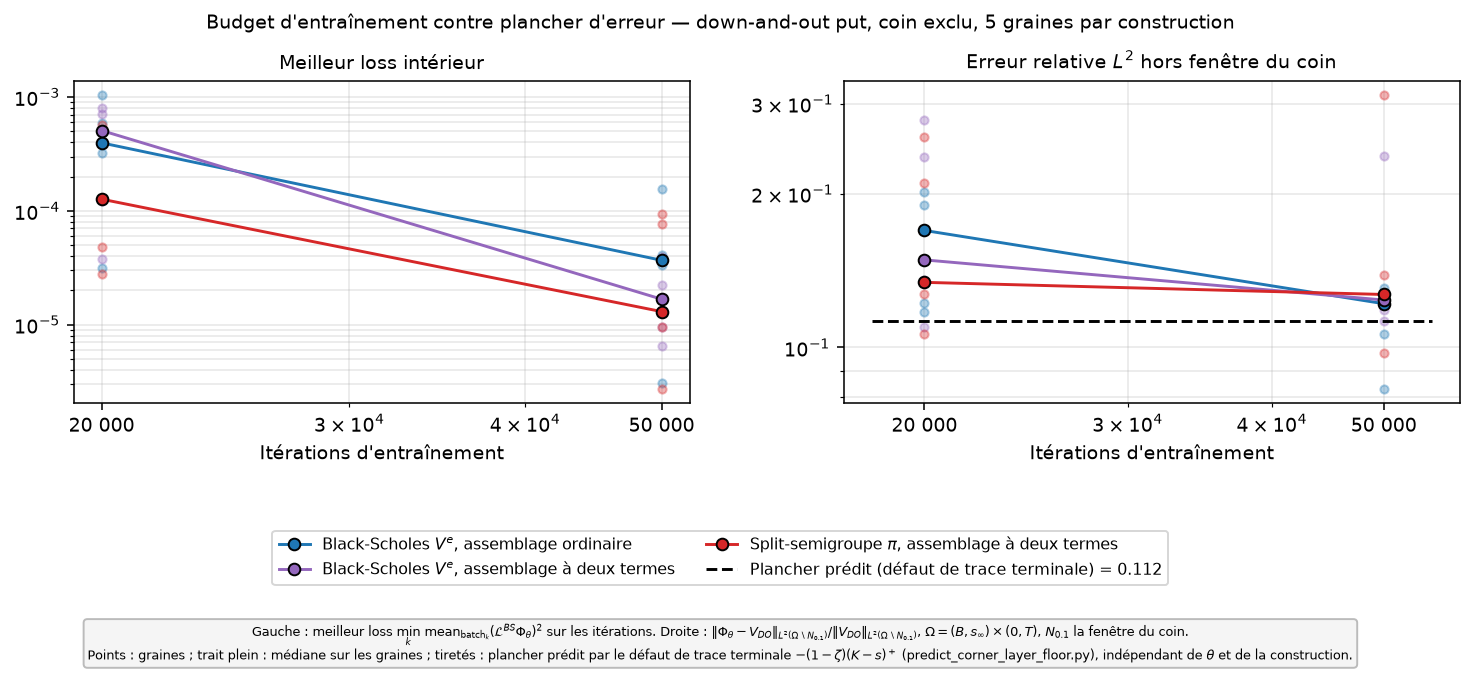
\includegraphics[width=\linewidth]{figures/fig3_budget_vs_plancher.png}
\caption{\mesure\ Budget d'entraînement contre erreur, de $20\,000$ à $50\,000$
itérations (mêmes graines, même machine, même nombre de threads). Le
meilleur loss intérieur décroît d'un facteur $11$, $30$ et $10$ ; l'erreur
relative sur $\Omega\setminus N_{0.1}$ d'un facteur $1.4$, $1.2$ et $1.05$
seulement, vers une valeur commune $0.12$--$0.13$. Tiretés : le plancher
prédit de la figure~\ref{fig:plancher}, $0.112$.}
\label{fig:budget}
\end{figure}

\paragraph{Le plancher est le défaut de trace terminale de l'ansatz.}
\etabli\ Pour les trois constructions, $g_1(s,T)=0$ et $h(s,T)=(K-s)^+$,
donc
\[
\Phi_\theta(s,T)=\zeta\!\left(\tfrac{s-B}{\epscoin}\right)(K-s)^+,
\qquad
\delta(s)=\Phi_\theta(s,T)-(K-s)^+=-\Big(1-\zeta\!\left(\tfrac{s-B}{\epscoin}\right)\Big)(K-s)^+ ,
\]
un défaut porté par $[B,B+\epscoin]$, égal à $-(K-B)=-0.4$ en $s=B^+$,
\emph{indépendant de $\theta$ et de $h$}. Il est forcé par l'exactitude de la
condition de barrière ($\zeta(0)=0$) jointe à l'incompatibilité des données au
coin ($\VDO(B,t)=0$ pour $t<T$, $\VDO(s,T)\to K-B$ quand $s\to B^+$). Si le
résidu intérieur était nul et les données de barrière et de far-field
exactes, l'erreur $w=\Phi_\theta-\VDO$ serait la solution de $\LBS w=0$,
$w(B,\cdot)=0$, $w(\cdot,T)=\delta$, c'est-à-dire le prix de l'option
down-and-out de payoff $\delta$, donné par le principe de réflexion
(\codepath{diagnostic_scripts/predict_corner_layer_floor.py}, quadrature
vérifiée contre la forme close à $8\times10^{-9}$).

\begin{figure}[htbp]
\centering
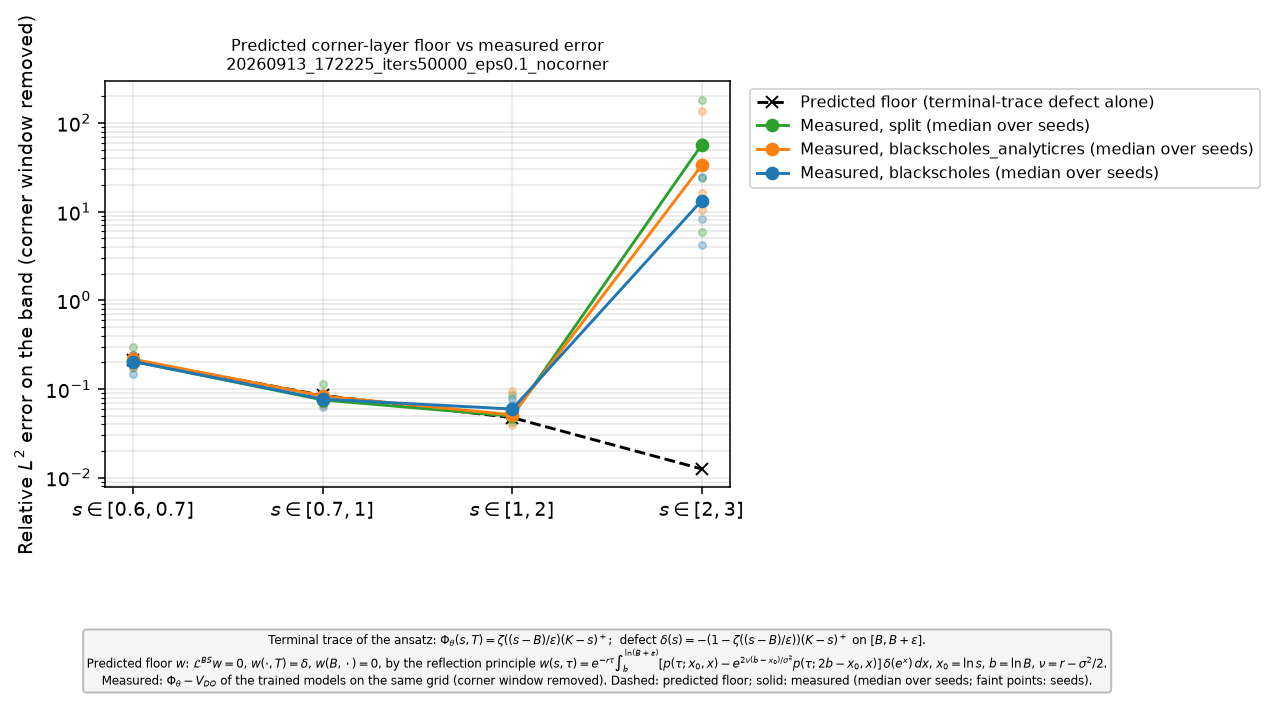
\includegraphics[width=\linewidth]{figures/fig4_plancher_predit_vs_mesure.png}
\caption{\mesure\ Erreur relative par tranche de $s$ (tout $t$, fenêtre
$N_{0.1}$ retirée) : plancher prédit par $\delta$ seul, sans réseau et sans
construction (tiretés noirs), contre les erreurs mesurées des quinze runs
(médianes en trait plein, graines en points). Sur $[0.6,0.7]$, $[0.7,1]$ et
$[1,2]$ : prédit $0.210$, $0.085$, $0.047$ ; mesuré $0.204$--$0.216$,
$0.075$--$0.083$, $0.049$--$0.059$. La tranche $[2,s_\infty]$ est une
composante distincte (far-field non contraint, dépendante de la graine), non
expliquée par $\delta$.}
\label{fig:plancher}
\end{figure}

\begin{figure}[htbp]
\centering
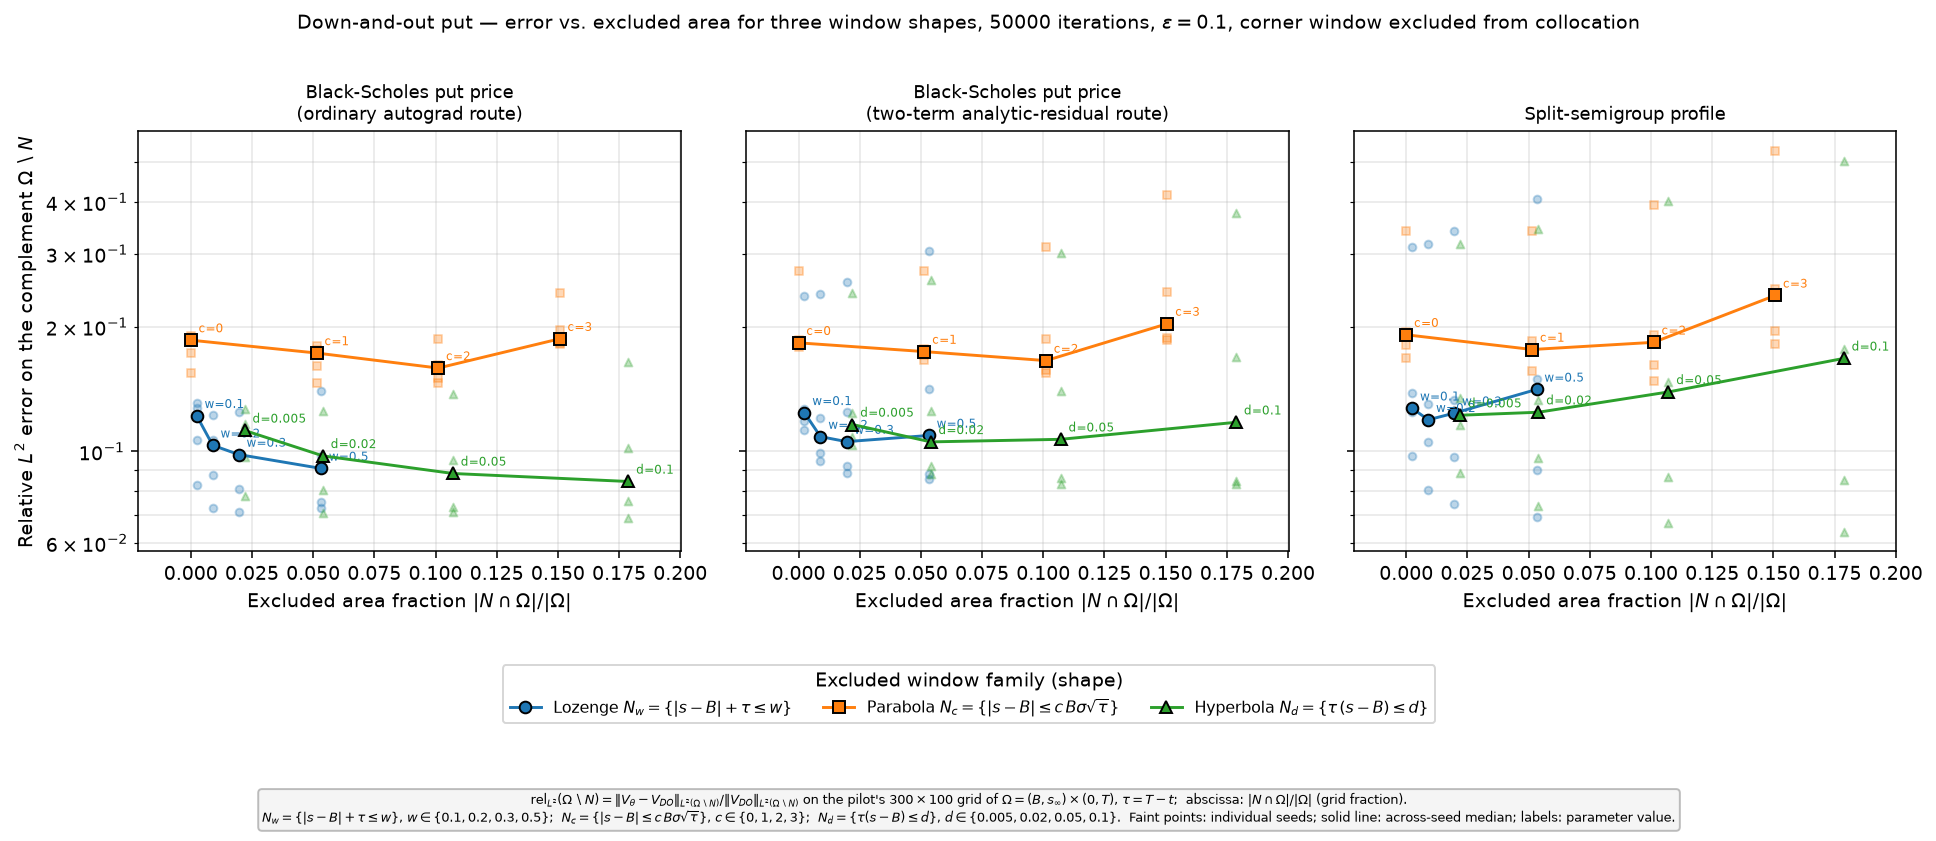
\includegraphics[width=\linewidth]{figures/fig5_balayage_fenetre.png}
\caption{\mesure\ Contrôle : erreur relative sur le complément d'une fenêtre
exclue, pour trois formes de fenêtre autour du coin, en fonction de l'aire
exclue. Aucune forme ne fait décroître l'erreur : le plancher n'est pas un
artefact de la fenêtre $N_{0.1}$ ; il est diffusé depuis la couche
$[B,B+\epscoin]$ vers l'intérieur, comme $w$ le prédit.}
\label{fig:fenetre}
\end{figure}

\section*{Conclusion}

Les trois constructions atteignent, à cinq graines, budget suffisant et
machine fixée, la même erreur à la dispersion entre graines près
(figures~\ref{fig:erreur-vs-temps} à \ref{fig:par-graine}) ; cette erreur
est un plancher que l'entraînement ne franchit pas
(figure~\ref{fig:budget}), prédit à $10$ pour cent près par le défaut de trace
terminale $-(1-\zeta)(K-s)^+$, commun aux trois puisque toutes vérifient
$h(\cdot,T)=(K-s)^+$ (figure~\ref{fig:plancher}). Tant que l'ansatz est
$\zeta h$, la fonction terminale $h$ n'est pas observable dans l'erreur ; le
choix entre constructions ne peut donc pas se faire sur la précision. Il
peut se faire sur le coût par itération ($V^e$ : $0.05$--$0.08$ s ; $\pi$ :
$1.0$ s, la quadrature étant recalculée à chaque appel), sur la régularité au
strike (courbure de $V^e$ en forme close ; plancher de quadrature de $\pi$
pour $\tau<1.2\times10^{-4}$) et sur la généricité ($\pi$ ne suppose pas
l'opérateur résolu), en le disant comme tel.

\end{document}
